\chapter{Regression, correlation and hypothesis testing}

\section{PMCC}
\begin{itemize}
	\item Measures the strength of \textbf{linear} correlation
	\item $r =\dfrac{\sum\left(x_{i}-\bar{x}\right)\left(y_{i}-\bar{y}\right)}{\sqrt{\sum\left(x_{i}-\bar{x}\right)^{2} \sum\left(y_{i}-\bar{y}\right)^{2}}}$ \textbf{(not needed for the exam)}
\end{itemize}

\section{Converting to linear form}
\subsection{Commenting on appropriateness}
\begin{itemize}
	\item \dots gives a linear relationship between \dots
	\item PMCC is close to $1$ or $-1$ which supports the use of a linear model
\end{itemize}

\section{Hypothesis test for zero linear correlation}
\subsection{Template}
\begin{itemize}
	\item $H_0$: $\rho = 0$
	\item $H_1$: $\rho \neq 0$ (two tailed) / $\rho > 0$ (right tail) / $\rho < 0$ (left tail)
	\item Sample size = $\dots$
	\item Significance level = $\dots$
	\item The critical value of $r$ for this test is $\dots$
	\item The observed value of $r$ is $\dots$
	\item $\dots < \dots$ so the observed value of $r$ is inside / outside the critical region
	\item So reject / accept $H_0$
	\item Conclusion
\end{itemize}




%\subsection{Sample variance}
%\begin{itemize}
%	\item $S^2=\dfrac{\Sigma(x_i-\overline{x})^2}{n-1}=\dfrac{1}{n-1}(\Sigma x_i^2-\overline{x}^2n)=\dfrac{1}{n-1}(\Sigma x_i^2-\dfrac{(\Sigma x)^2}{n})$
%\end{itemize}



\chapter{Conditional probability}
\section{Conditional probability formula}
\begin{itemize}
	\item $P(A|B) = \dfrac{P(A \cap B)}{P(B)}$
\end{itemize}
\section{Principle of inclusion-exclusion}
\begin{itemize}
	\item $P(A\cup B)=P(A)+P(B)-P(A\cap B)$
\end{itemize}

\chapter{The normal distribution}
\section{Notation}
\begin{itemize}
	\item $X \sim N(\mu,\sigma^2)$
	\item $\mu$ = mean of the population
	\item $\sigma^2$ = \textbf{variance} of the data
\end{itemize}
\section{Properties}
\begin{itemize}
	\item The data is \textbf{continuous}
	\item Has parameters $\mu$ (mean) and $\sigma^2$ (variance)
	\item Is symmetrical: mean = median = mode
	\item Has a bell-shaped curve with asymptotes at each end
	\item Total area under the curve = $1$
	\item Has points of inflection at $\mu+\sigma$ and $\mu-\sigma$
\end{itemize}

\section{Estimating probabilities}
\begin{itemize}
	\item $68\%$ of observations lie within $\pm 1$ standard deviation of the mean
	\item $95\%$ of observations lie within $\pm 2$ standard deviation of the mean
	\item $99.8\%$ of observations lie within $\pm 3$ standard deviation of the mean
\end{itemize}
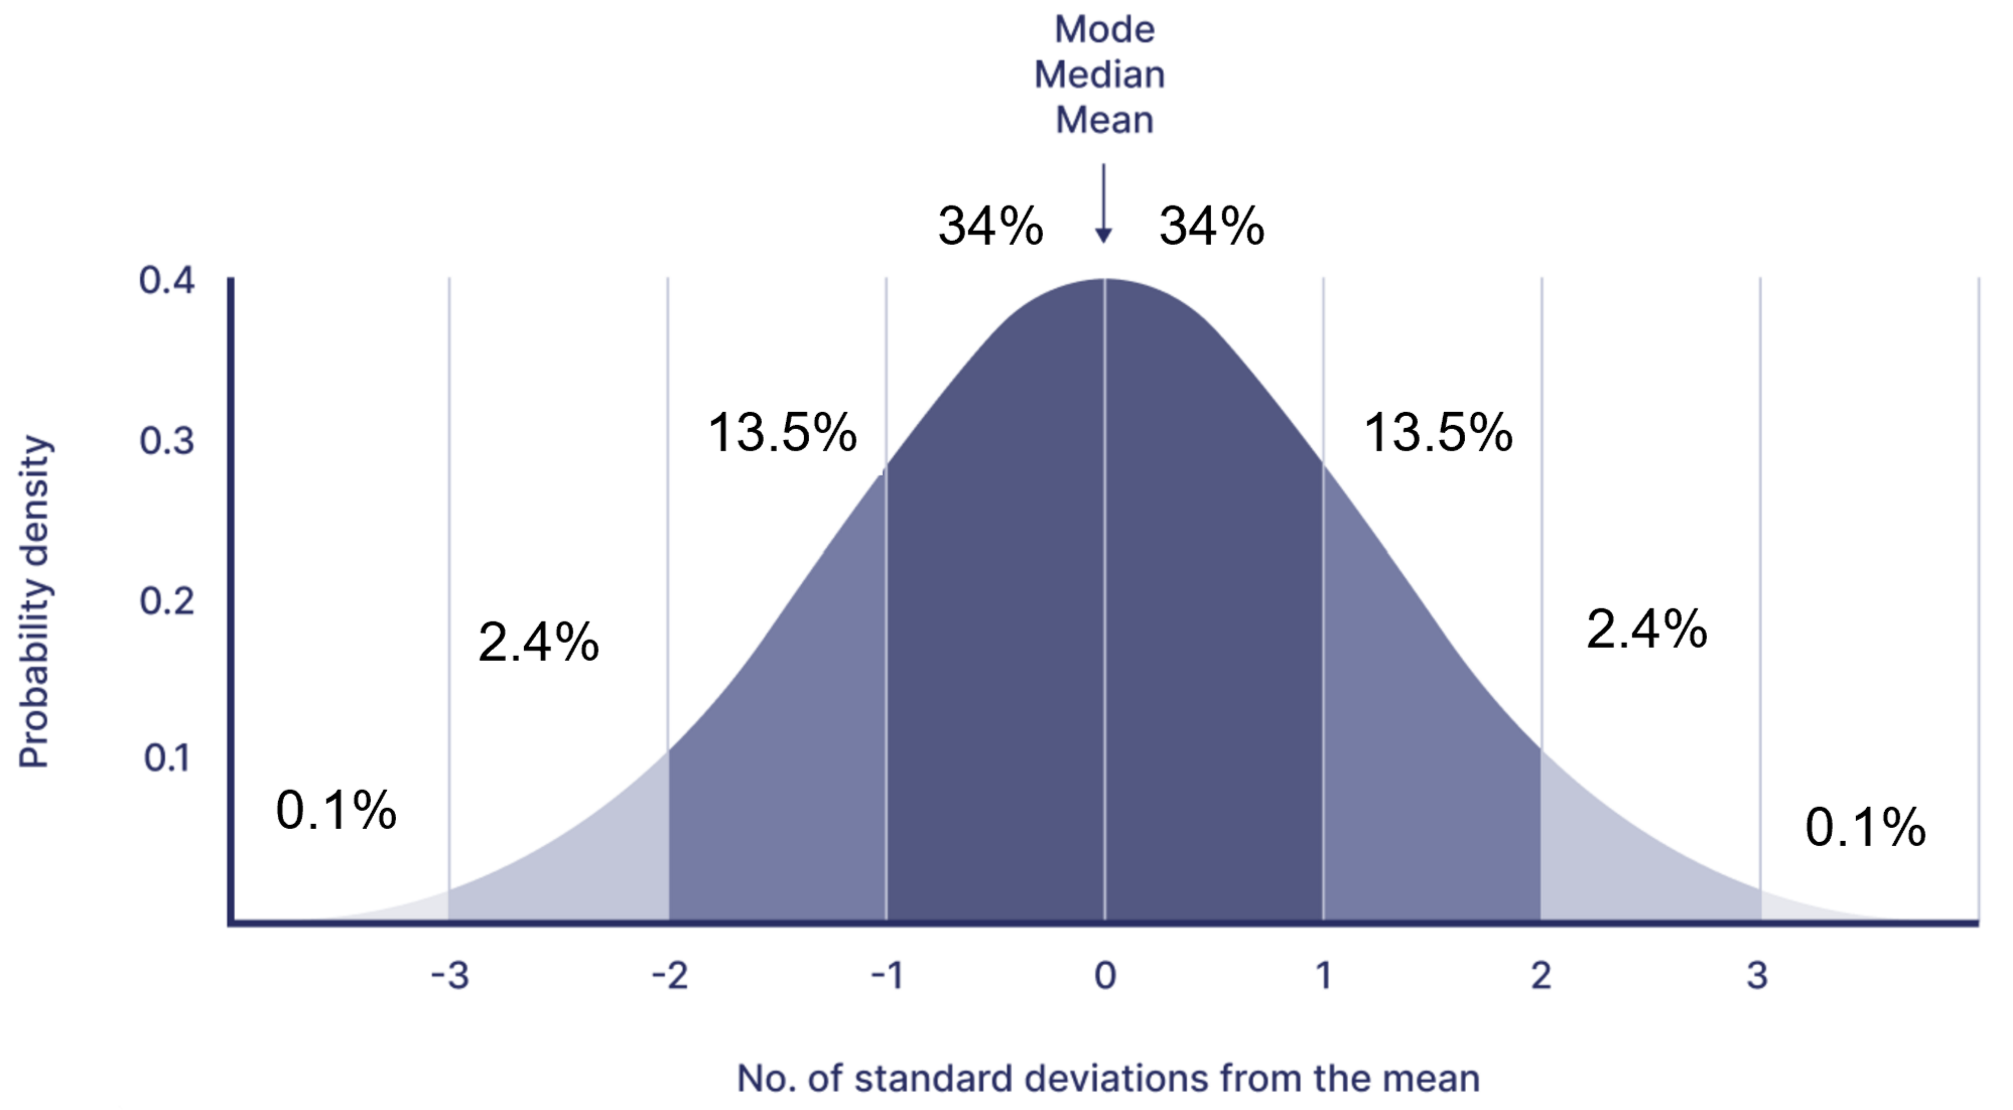
\includegraphics[width=0.7\linewidth]{images/normal_estimate}

\section{Approximation of binomial distribution}
If $n$ is large ($n\geq35$) and $p$ is close to $0.5$, then $X \sim B(n,p)$ can be modelled as $$Y \sim N(np, np(1-p))$$
\subsection{Approximations}
\begin{itemize}
	\item $\text{P}(X\geq a)\approx \text{P}(Y\geq [a-0.5])$
	\item $\text{P}(X=a)\approx \text{P}([a-0.5]<Y<[a+0.5])$
	\item $\text{P}(X \leq a)\approx \text{P}(Y\leq [a+0.5])$
\end{itemize}


\section{Sample mean}
If $n$ is large enough ($n\geq35$) and $X\sim N(\mu, \sigma^2)$, then sample mean $\overline{X}$ is normally distributed: $$\overline{X} \sim N\left(\mu, \frac{\sigma^2}{n}\right)=N\left(\mu, \left(\frac{\sigma}{\sqrt{n}}\right)^2\right)$$